\mychapter{2}{sBLISS}
\label{chap:BLISS_sBLISS}
Breaks Labeling In Situ and Sequencing or `BLISS' was introduced in 2017 \cite{yan2017bliss} and has since been re-made into in-Suspension Breaks Labeling In Situ and Sequencing or `sBLISS' \cite{bouwman2020genome}. sBLISS serves as a method to identify double-stranded breaks (DSBs) in a genome. From a bioinformatic perspective, this technology leverages Unique Molecular Identifiers (UMIs) to identify unique double stranded breaks as well as their location in the genome. See \autoref{fig:sbliss_workflow} for an overview of the protocol from a lab perspective.

\section{Scan for Matches \label{sec:scan_for_matches}}
The sBLISS pipeline utilizes scan\_for\_matches as an element of it's method, however the installation of this has become quite difficult. In order to install it on our local computer we had to use an old version of linux, do the installation, then export the file from /usr/bin/. This file was then transferred to the computer with a current linux version and manually inserted into it's /usr/bin/. This is not an ideal solution as it is quite difficult to replicate, if at all.\\
I have created a bash based script to substitute the scan\_for\_matches component used in the standard sBLISS pipeline. The sBLISS pipeline shipped with this toolbox comes equipped with this new method, however the old method remains in the main script, it is simply commented out.

\section{Adaptor anatomy \label{sec:sBliss_adaptors}}
\begin{itemize}
\item \textbf{T7 promoter sequence} - used for amplification
\item \textbf{RA5 adaptor} - Necessary for sequencing
\item \textbf{UMI} - Allows us to remove duplicates while processing the sequenced data
\item \textbf{Sample Barcode} - Used for demultiplexing (if required) and to quality control the data processing
\end{itemize}
Without going into details (yet) the T7 and RA5 elements are of no use in data processing, in which case they will have to be `trimmed' from the sequencing (fastq) files. It is likely that these have already been removed \todo{explain how to check this}.\\
The UMI and sample barcode are relevant, and recurring in the bioinformatic analysis. It is very important to know the length of each of these adaptors. Looking at the box below you can see a simplified example of a fastq file line. We have the header which provides a name and an contain some information between the colons (not always). For now this information is not relevant. The importance is to note the highlighted areas of the sequence. In this example the sample SRR11119500 has a UMI of AAAGGNAA and a sample barcode of CATCACGC. The UMI will be unique for each line of the fastq file while the sample barcode will always be the same. Knowing the sample barcode is essential for the proper functioning of the sBLISS pipeline as the program must know the barcode associated to each sample. By knowing the length and format of the adaptor we are capable of finding the sample barcode if it is no explicitly provided. In this experiment we knew that the UMI preceded the barcode and the UMI was of 8 nucleotides long, with the sample barcode having the same length. From this we could establish what the sample barcode was by taking nucleotides 8-16 of each line of the fastq file and checking which was the most recurring pattern. We have to check the entire file as there may be mismatches. This will be covered in more details later, however know that the pipeline will allow for no more than 1 mismatched nucleotide in a sample barcode.

\begin{formal}
@SRR11119500.1:::1:::length=76\\
\hlorange{AAAGGNAA}\hlsteelblue{CATCACGC}AGTGGTATTATAAGAAC[...]
\end{formal}

\begin{figure}
\centering
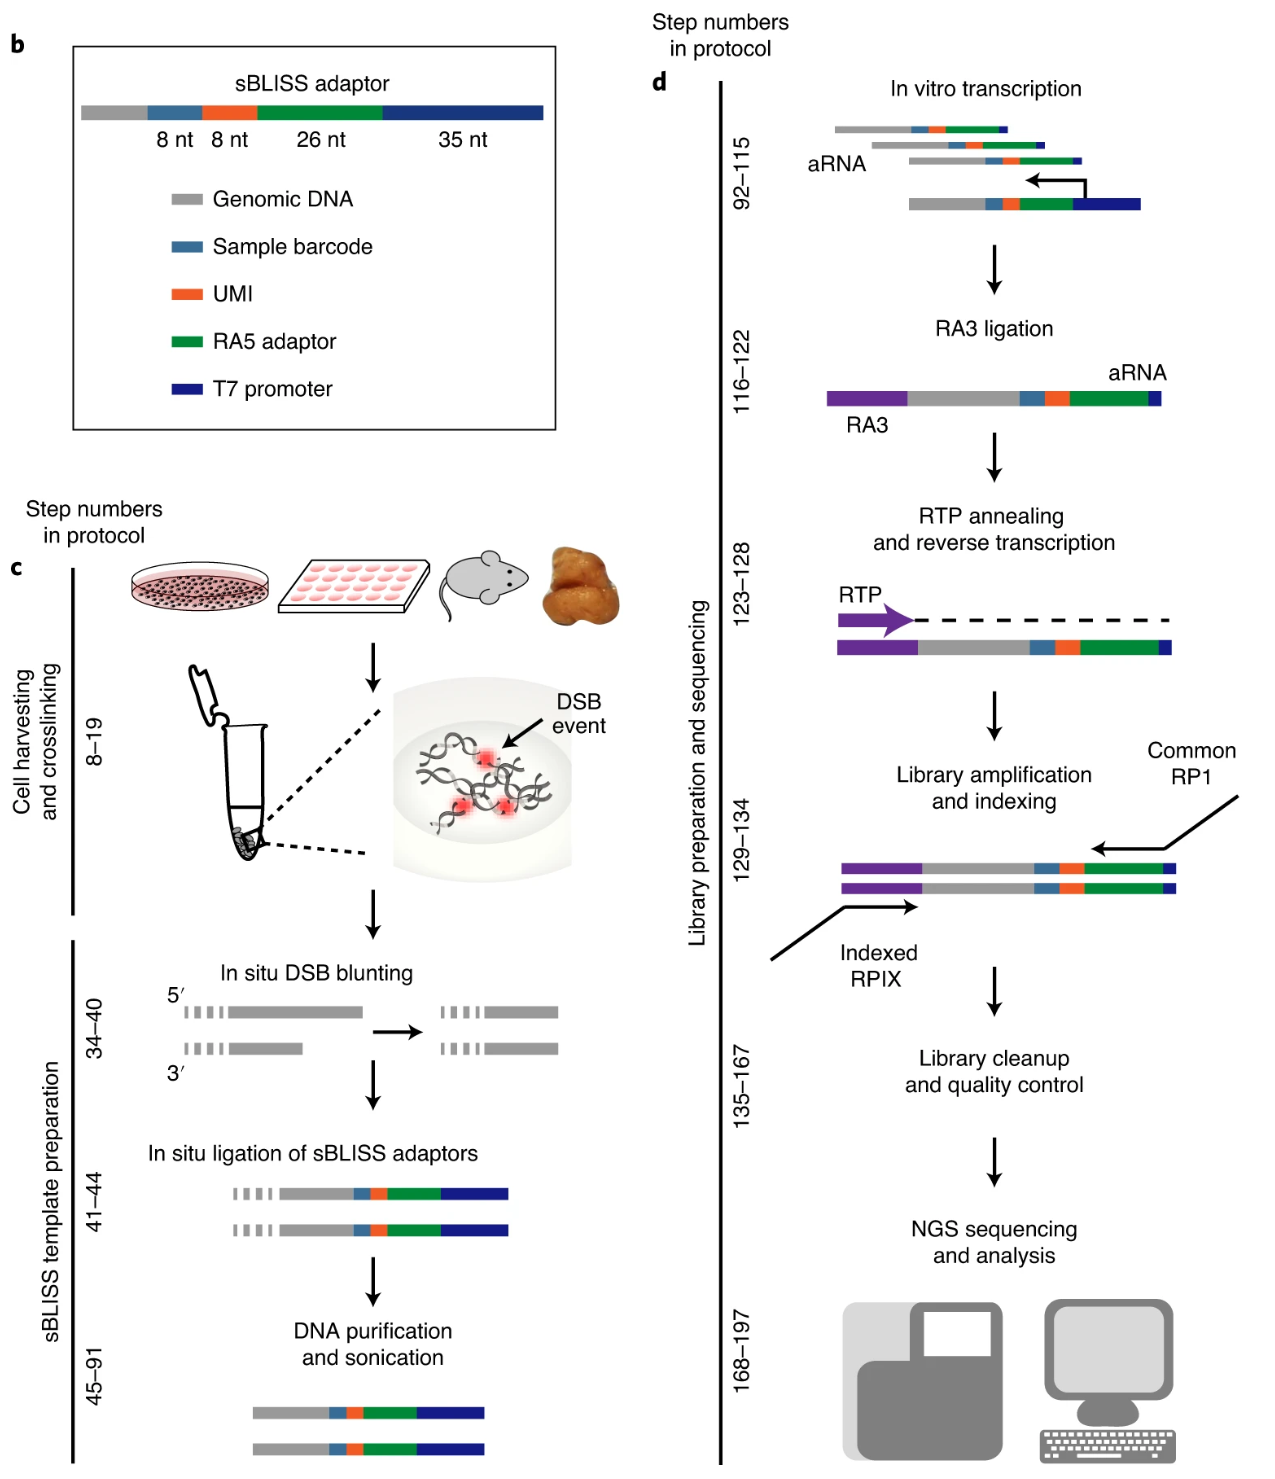
\includegraphics[width=12cm, height=14cm]{figures/sBLISS_workflow.png}
\caption{b, Sequence structure of the sBLISS adaptor. c and d, Step-by-step scheme of the protocol.\\
Figure from \protect\cite{bouwman2020genome} - figure 1}
\label{fig:sbliss_workflow}
\end{figure}

\section{Verify Fastq files \label{sec:sbliss_check_fastq}}
Fastq files can come in a variety of formats \autoref{sec:Fastq_files}, the sBLISS pipeline requires a relatively specific format. This is discussed in a github issue (\url{https://github.com/BiCroLab/blissNP/issues/6}). Essentially, some fastq files, especially those downloaded form NCBI or other repositories, may be incorrectly formatted for this pipeline. To check this, you can simply open the fastq file (you may have to extract it first). Open the fastq file using the `glogg' software \autoref{sec:glogg}. If you observe a format where the header (see the box in \autoref{sec:sBliss_adaptors} above) contains colons, then the format is likely to be correct. In the case where it contains no colons or fails a check (detailed below), you can run the `fix\_fastq\_format.sh' script with the following method:\\
\begin{enumerate}
\item Move to directory with the script
\begin{lstlisting}
cd seq_toolbox/sbliss/
\end{lstlisting}
\item Launch the script while providing a path to the directory
\begin{lstlisting}
bash fix_fastq_format.sh path_to_data
\end{lstlisting}
\end{enumerate}
Once the script is complete the directory you gave will contain files with the term 'fixed' appended to them. You should move these files to an alternate folder/location.\\
Additionally there is a check implemented on the script where an incorrect file format will usually result in a blank file. This is not a fool proof check though it does serve as an indication of a possible issue in the file format. The error will read
\begin{displayquote}
Error: r2.2b.aln.fq is empty. This may be due to incorrect fastq file format. See the section of the guide titled 'sBLISS check your Fastq files'. Terminating script.
\end{displayquote}
If you observe this error, it is likely that the fastq format is incorrect. If this is not the case contact the author of seq-toolbox for advice.

\section{Data processing \label{sec:sbliss_dta_process}}
The pipeline is broken down in several components. The provided guide is meant to help you run it yourself provided that all elements are already installed on the computer. If this is not the case, see the installation section \autoref{chap:Install}. To simplify the task the pipeline operates via what is called a sample file, as seen in table \autoref{tab:sample_file}. The first column must be identical to the fastq file name. For example SRR11119500's file name would be SRR11119500.fastq.gz, with the gz standing for a gnu zipped archive, essentially a type of compression. The second column is whatever name the user desires, the results will be saved under this name. The adaptor is discussed and explained in the previous section. The number of mismatches is also discussed, and though it is possible to adjust it I would strongly recommend not to.\\
Note that currently this pipeline only works on human and mouse. If you have other organisms you'd like to use please let me know and I'll see what I can do. \todo{finish implementing celegans}

\begin{table}
\caption{Table illustrating the sample file, which would normally be in a csv format. The columns are as follows: Sample name (as given to the fastq file), treatment name (can be whatever the use desires), sample barcode (see \autoref{sec:sBliss_adaptors}, genome, number of allowed mismatches for the sample barcode.} 
\begin{tabular}{|c c c c c|}
\hline
 SRR11119500 & TK6\_DMSO\_Rep1 & CATCACGC & human & 1\\ 
 \hline
 SRR11119501 & TK6\_ETO\_Rep1 & GTCGTCGC & human & 1\\
 \hline
 SRR11119502 & TK6\_DMSO\_Rep2 & CATCACGC & human & 1\\
 \hline
 SRR11119503 & TK6\_ETO\_Rep2 & GTCGTCGC & human & 1\\
 \hline
\end{tabular}
\label{tab:sample_file}
\end{table}

Once this sample file has been build and saved as a csv file (comma-separated values) \todo{How to save a file from excel to csv?}. we can get into the organization of the folder where the work will be done.\\
\textbf{IMPORTANT: }The pipeline is set-up for either SE or PE. In a PE (paired-end) condition only one line for the two files is required. If we assume a paired-end file called OB1\_1.fastq.gz and OB1\_2.fastq.gz, then the sample file should only contain an entry for OB1. Note that the sample barcode in a PE case is only found in the forward file (\_1).

\subsection{Bash script for sample file}
If a user only has the fastq files and not the sample barcodes, these can be found through the fastq files. The sample barcode is seen from the 8th nucleotide to the 16th, as shown in \autoref{sec:sBliss_adaptors}. However not all sequences will be correct, some will have mismatches, therefore the best approach is to go through the entire fastq file, retrieve the 8th to 16th nucleotide, and using these, check which sequence appears most often. This sequence of 8 nucleotides will be the sample barcode. A bash script was created to accomplish this. It is called `extract\_sample\_barcode.sh'. When calling this script simply give the directory where the data is located and it will output a file containing the identified sample barcode for each file ending in `fastq.gz'.

Within the sBLISS folder in the computer you will see four folders, titled `bin', `python', `runs', `.git', and `test\_TK6\_hg19'. This last folder is the test folder used to set-up this pipeline. You should create your own folder, call it whatever you'd like, and store your sample file here.\\
From here on the steps to follow will utilize the terminal. To open the terminal press super+T on the keyboard, now follow the instructions below. For more information on the terminal see \autoref{sec:terminal}.\\
\begin{enumerate}
\item Start by going into the sBLISS directory. The cd (change directory) command is used
\begin{lstlisting}
cd seq_toolbox/sbliss/
\end{lstlisting}

\item Activate the environment that will be used. See \autoref{sec:conda} for more information on conda environments.
\begin{lstlisting}
conda activate seq-toolbox
\end{lstlisting}

\item Prepare the patterns using the sample sheet. Note that I am using the `test\_TK6\_hg19' file name, you will have to use your own folder name.\\
\todo{May be unnecessary with the new scan for matches method.}
\begin{lstlisting}
bash bin/prepare_pattern.sh test_TK6_hg19/sample_sheet.csv
\end{lstlisting}
If this worked you will notice new files in your folder, there should be one new file per row in your sample file.

\item Prepare the run. Here you can give a name to the run (run\_name), you also need to provide the path to the data. You may have it in your folder, so for example writing `test\_TK6\_hg19/data/' would work provided that all the fastq.gz files are located there. If your data is on a hard drive, make sure it is plugged in and navigate to that data. The way you reach a hard drive via command line changed from one computer to another. In this case we do the following: `/media/yohanl/name\_of\_harddrive'.
\begin{lstlisting}
bash bin/prepare_run.sh test_TK6_hg19/sample_sheet.csv run_name path_to_data
\end{lstlisting}
If this worked there should be a file in the `runs' folder with the name you provided.\\
\textbf{IMPORTANT: The code looks for files with the extension `.fastq.gz' so if the extension is currently `.fq.gz' manually adjust the file extensions to be `fastq.gz'}\todo{Yohan: Adjust this in the code, make it not a problem.}
\item The last step is to launch the run
\begin{lstlisting}
bash runs/run_name.sh
\end{lstlisting}
This should start the pipeline. Depending on the number of files and the size of these files it may take several hours, if not a whole day. Ensure that the computer is plugged in. You can now let it do it's thing. You will know when it is finished once the prompt on the terminal has become green. The pipeline automatically generates some text to state where it is located in the pipeline. Note that the green prompt simply indicates that the terminal is no longer busy, which could mean that the pipeline has finished, or it has encountered an error. In the case of an error the text in the terminal should state the error. 
\end{enumerate}

The results will be located in the folder you created. The results will be split into folders which carry the names you used in the sample file. Each of these folders is structured the same way.\\
The three first files are `chr-loc-countDifferentUMI.bed', `chr-loc-strand-umi-pcr.tsv', and `summary.txt.'\\
The summary file contains the summary of the analysis, the main interest being the number of UMIs found and the number of DSBs found. The .tsv file represents the results based on the number of UMIs identified, while the .bed file is the same set of results but without the deduplicated UMIs. The bed file is the one that will be used for subsequent analyses. Note that these files are relatively large and cannot be opened by conventional programs, if you do so it may crash the computer. You can take a look inside the files by opening with a program called `glogg'. Just right-click the file, then open with glogg \autoref{sec:glogg}.\\
Another folder of importance is the QC results. Two quality control methods are used in this pipeline, fastqc and fastq screen. Each of these are explained in their respective sections of this report, see \autoref{sec:fastqc} and \autoref{sec:Fast_Screen} respectively.

\section{Peak calling \label{sec:bliss_peak_calling}}
For the full breakdown of peak calling and what it is check \autoref{sec:peak_call}\\
In this section we cover the limitations of peak calling in regards to sBLISS.

\section{Data analysis \label{sec:sBLISS_dta_analysis}}
\textbf{NOT AUTOMATED YET} - in principal it will operate on a sample file basis, though this sample file will need some adjustments, specifically what should be bound together in certain analysis. \todo{This area}
